\documentclass[14pt]{extbook}
\usepackage{multicol, enumerate, enumitem, hyperref, color, soul, setspace, parskip, fancyhdr} %General Packages
\usepackage{amssymb, amsthm, amsmath, bbm, latexsym, units, mathtools} %Math Packages
\everymath{\displaystyle} %All math in Display Style
% Packages with additional options
\usepackage[headsep=0.5cm,headheight=12pt, left=1 in,right= 1 in,top= 1 in,bottom= 1 in]{geometry}
\usepackage[usenames,dvipsnames]{xcolor}
\usepackage{dashrule}  % Package to use the command below to create lines between items
\newcommand{\litem}[1]{\item#1\hspace*{-1cm}\rule{\textwidth}{0.4pt}}
\pagestyle{fancy}
\lhead{Progress Quiz 4}
\chead{}
\rhead{Version A}
\lfoot{6286-1986}
\cfoot{}
\rfoot{Fall 2020}
\begin{document}

\begin{enumerate}
\litem{
Choose the graph of the equation below.\[ f(x) = \frac{1}{(x - 1)^2} + 1 \]\begin{enumerate}[label=\Alph*.]
\begin{multicols}{2}\item 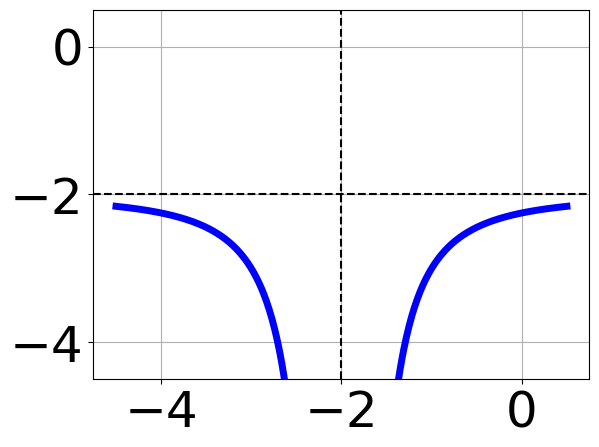
\includegraphics[width = 0.3\textwidth]{../Figures/rationalEquationToGraphAA.png}\item 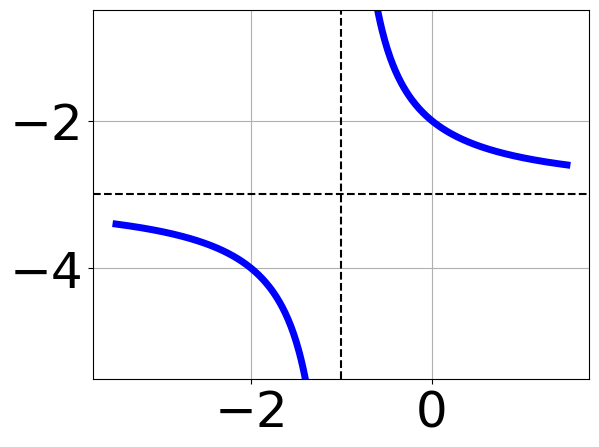
\includegraphics[width = 0.3\textwidth]{../Figures/rationalEquationToGraphBA.png}\item 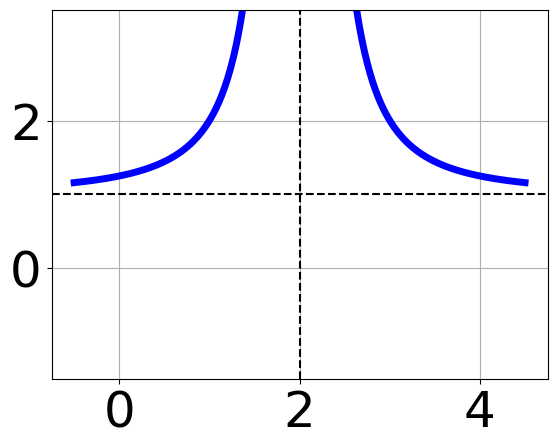
\includegraphics[width = 0.3\textwidth]{../Figures/rationalEquationToGraphCA.png}\item 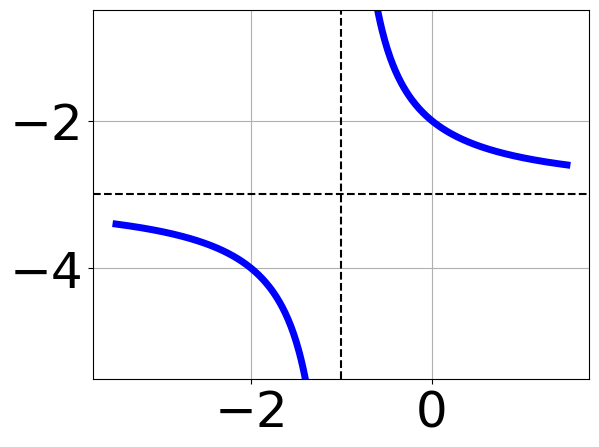
\includegraphics[width = 0.3\textwidth]{../Figures/rationalEquationToGraphDA.png}\end{multicols}\item None of the above.
\end{enumerate} }
\litem{
Choose the equation of the function graphed below.
\begin{center}
    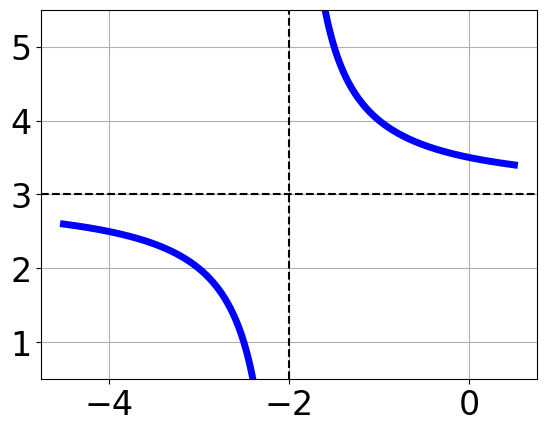
\includegraphics[width=0.5\textwidth]{../Figures/rationalGraphToEquationA.png}
\end{center}
\begin{enumerate}[label=\Alph*.]
\item \( f(x) = \frac{-1}{(x + 3)^2} - 1 \)
\item \( f(x) = \frac{-1}{x + 3} - 1 \)
\item \( f(x) = \frac{1}{x - 3} - 1 \)
\item \( f(x) = \frac{1}{(x - 3)^2} - 1 \)
\item \( \text{None of the above} \)

\end{enumerate} }
\litem{
Solve the rational equation below. Then, choose the interval(s) that the solution(s) belongs to.\[ \frac{60}{-72x -60} + 1 = \frac{60}{-72x -60} \]\begin{enumerate}[label=\Alph*.]
\item \( x \in [0.4,2.8] \)
\item \( x_1 \in [-1.5, -0.1] \text{ and } x_2 \in [-1.83,0.17] \)
\item \( x_1 \in [-1.5, -0.1] \text{ and } x_2 \in [-0.17,3.83] \)
\item \( x \in [-0.83,0.17] \)
\item \( \text{All solutions lead to invalid or complex values in the equation.} \)

\end{enumerate} }
\litem{
Determine the domain of the function below.\[ f(x) = \frac{4}{20x^{2} +x -30} \]\begin{enumerate}[label=\Alph*.]
\item \( \text{All Real numbers.} \)
\item \( \text{All Real numbers except } x = a \text{ and } x = b, \text{ where } a \in [-4.25, -0.25] \text{ and } b \in [1.2, 2.2] \)
\item \( \text{All Real numbers except } x = a \text{ and } x = b, \text{ where } a \in [-20, -17] \text{ and } b \in [30, 32] \)
\item \( \text{All Real numbers except } x = a, \text{ where } a \in [-20, -17] \)
\item \( \text{All Real numbers except } x = a, \text{ where } a \in [-4.25, -0.25] \)

\end{enumerate} }
\litem{
Solve the rational equation below. Then, choose the interval(s) that the solution(s) belongs to.\[ \frac{6x}{5x -5} + \frac{-4x^{2}}{20x^{2} -35 x + 15} = \frac{-7}{4x -3} \]\begin{enumerate}[label=\Alph*.]
\item \( x \in [-1.83,-1.71] \)
\item \( x_1 \in [0.84, 1.05] \text{ and } x_2 \in [-4.81,0.19] \)
\item \( x_1 \in [0.84, 1.05] \text{ and } x_2 \in [-1,4] \)
\item \( x \in [0.7,0.85] \)
\item \( \text{All solutions lead to invalid or complex values in the equation.} \)

\end{enumerate} }
\litem{
Choose the equation of the function graphed below.
\begin{center}
    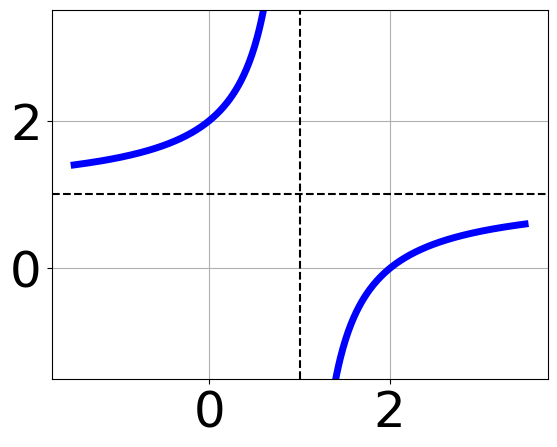
\includegraphics[width=0.5\textwidth]{../Figures/rationalGraphToEquationCopyA.png}
\end{center}
\begin{enumerate}[label=\Alph*.]
\item \( f(x) = \frac{-1}{x + 2} + 3 \)
\item \( f(x) = \frac{1}{(x - 2)^2} + 3 \)
\item \( f(x) = \frac{-1}{(x + 2)^2} + 3 \)
\item \( f(x) = \frac{1}{x - 2} + 3 \)
\item \( \text{None of the above} \)

\end{enumerate} }
\litem{
Choose the graph of the equation below.\[ f(x) = \frac{-1}{(x + 3)^2} + 3 \]\begin{enumerate}[label=\Alph*.]
\begin{multicols}{2}\item 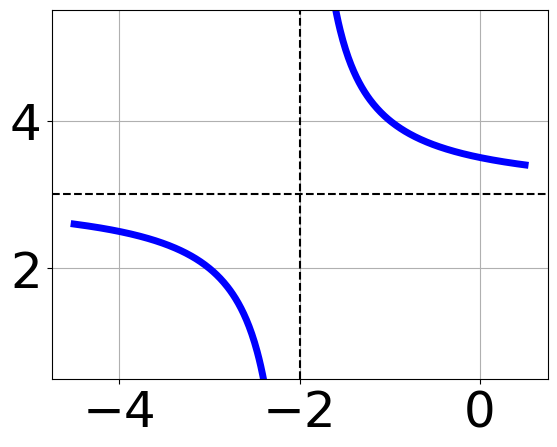
\includegraphics[width = 0.3\textwidth]{../Figures/rationalEquationToGraphCopyAA.png}\item 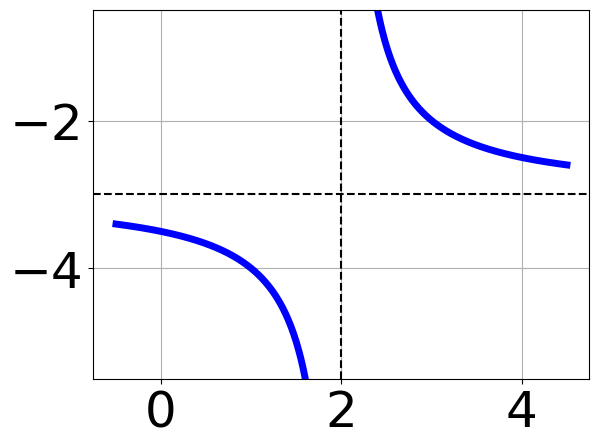
\includegraphics[width = 0.3\textwidth]{../Figures/rationalEquationToGraphCopyBA.png}\item 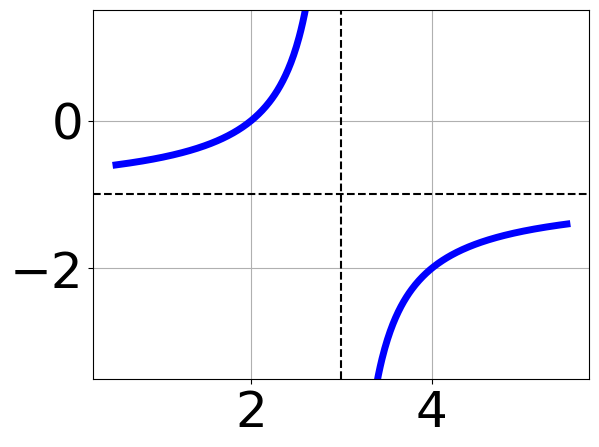
\includegraphics[width = 0.3\textwidth]{../Figures/rationalEquationToGraphCopyCA.png}\item 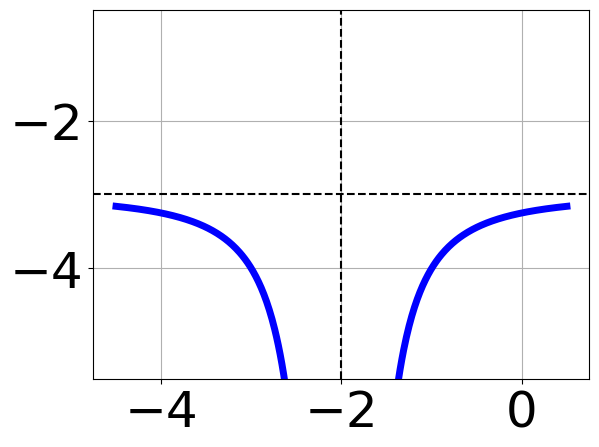
\includegraphics[width = 0.3\textwidth]{../Figures/rationalEquationToGraphCopyDA.png}\end{multicols}\item None of the above.
\end{enumerate} }
\litem{
Solve the rational equation below. Then, choose the interval(s) that the solution(s) belongs to.\[ \frac{9}{5x -8} + -5 = \frac{6}{-45x + 72} \]\begin{enumerate}[label=\Alph*.]
\item \( x_1 \in [-1.43, -0.9] \text{ and } x_2 \in [0.99,4.99] \)
\item \( x \in [-1.43,-0.9] \)
\item \( x_1 \in [1.62, 1.9] \text{ and } x_2 \in [0.99,4.99] \)
\item \( \text{All solutions lead to invalid or complex values in the equation.} \)
\item \( x \in [1.99,2.99] \)

\end{enumerate} }
\litem{
Solve the rational equation below. Then, choose the interval(s) that the solution(s) belongs to.\[ \frac{2x}{3x + 5} + \frac{-7x^{2}}{12x^{2} +29 x + 15} = \frac{4}{4x + 3} \]\begin{enumerate}[label=\Alph*.]
\item \( \text{All solutions lead to invalid or complex values in the equation.} \)
\item \( x \in [7.7,9.8] \)
\item \( x_1 \in [-3.1, -1.3] \text{ and } x_2 \in [6.38,9.38] \)
\item \( x \in [-2.1,3.3] \)
\item \( x_1 \in [-3.1, -1.3] \text{ and } x_2 \in [-7.67,-0.67] \)

\end{enumerate} }
\litem{
Determine the domain of the function below.\[ f(x) = \frac{6}{24x^{2} -48 x + 18} \]\begin{enumerate}[label=\Alph*.]
\item \( \text{All Real numbers except } x = a, \text{ where } a \in [17, 18.3] \)
\item \( \text{All Real numbers except } x = a \text{ and } x = b, \text{ where } a \in [-0.1, 0.8] \text{ and } b \in [1, 2.2] \)
\item \( \text{All Real numbers except } x = a, \text{ where } a \in [-0.1, 0.8] \)
\item \( \text{All Real numbers except } x = a \text{ and } x = b, \text{ where } a \in [17, 18.3] \text{ and } b \in [23.8, 25.4] \)
\item \( \text{All Real numbers.} \)

\end{enumerate} }
\end{enumerate}

\end{document}